\documentclass[10pt, svgnames, compress, red]{beamer}


%%%%%%%%%%%%% PACKAGE ESSENTIEL

\usepackage{lmodern}
\usepackage{palatino}
\usepackage[T1]{fontenc}
\usepackage[utf8]{inputenc}
\usepackage[english]{babel}

%%%%%%%%%%%%% PACKAGE FACULTATIF
\usepackage{multimedia}				% to use multimedia
\usepackage{graphics}				% to use graphics
\usepackage{subfigure}				% to use figure in figure
\hypersetup{pdfstartview={Fit}}
\graphicspath{{./images/}}		% to say where are image
% \RequirePackage{pageGardeEnsta}
% \usepackage[svgnames]{xcolor}
\usepackage{natbib}
\usepackage{caption}
\usepackage{appendixnumberbeamer}

%%%%%%%%%%%%% THEME
\mode<presentation>
\usetheme{Warsaw}
\usecolortheme{lily}
\useoutertheme[subsection=false]{smoothbars}
\useinnertheme{circles}
\useoutertheme{shadow}
\usefonttheme{serif}

%%%%%%%%%%%%%%%%%%%%%%%%%
\hypersetup{
%  pdfpagemode = FullScreen,% afficher le pdf en plein écran
  pdfkeywords = {militaire,formation,humaine},%
  pdfcreator  = {PDFLaTeX},%
  pdfproducer = {PDFLaTeX}%
}


%% Permet la non numérotation des pages en annexes pour réaliser des slides cachés
\expandafter\def\expandafter\insertshorttitle\expandafter{%
  \insertshorttitle\hfill\insertframenumber\,/\,\inserttotalframenumber}



%%%% Permet affiche en début de chaque section, les noms de sections et
%%%% noms de sous-sections de la section en cours.

\AtBeginSection[]{
  \begin{frame}
    \begin{center}{\Large Table of contents }\end{center}
    \tableofcontents[currentsection,hideothersubsections]
    \transdissolve[duration=0.1]
  \end{frame}

}

%%%%%%%%%%%%%%%
% \titlegraphic{%
% \begin{center}
%
% \end{center}}
%
% \setbeamertemplate{titlepage}{%
% \inserttitlegraphic}
\setbeamercolor{background canvas}{bg=Beige}
%%%%%%%%%%%%%%%%%



\setbeamertemplate{footline}{
\leavevmode%
\hbox{\hspace*{-0.06cm}
\begin{beamercolorbox}[wd=.2\paperwidth,ht=2.25ex,dp=1ex,center]{author in head/foot}%
	\usebeamerfont{author in head/foot}\insertshortauthor%~~(\insertshortinstitute)
\end{beamercolorbox}%
\begin{beamercolorbox}[wd=.6\paperwidth,ht=2.25ex,dp=1ex,center]{section in head/foot}%
	\usebeamerfont{section in head/foot}\insertshorttitle
\end{beamercolorbox}%
\begin{beamercolorbox}[wd=.2\paperwidth,ht=2.25ex,dp=1ex,right]{section in head/foot}%
	\usebeamerfont{section in head/foot}\insertshortdate{}\hspace*{2em}
	\insertframenumber{} / \inserttotalframenumber\hspace*{2ex}
\end{beamercolorbox}}%
\vskip0pt%
}
\bibliographystyle{plain}
% make bibliography entries smaller
\renewcommand*{\bibfont}{\footnotesize}
% If you have more than one page of references, you want to tell beamer
% to put the continuation section label from the second slide onwards
\setbeamertemplate{frametitle continuation}[from second]
% Now get rid of all the colours
\setbeamercolor*{bibliography entry title}{fg=black}
\setbeamercolor*{bibliography entry author}{fg=black}
\setbeamercolor*{bibliography entry location}{fg=black}
\setbeamercolor*{bibliography entry note}{fg=black}
% and kill the abominable icon
\setbeamertemplate{bibliography item}{}



%%%%%%%%%%%% TITRE

\institute{ENSTA Bretagne}
\subtitle{Final presentation}
\title{UML-DSimulator}
\subject{}
\author{IETA RIGAUD Michaël}
\logo{
\includegraphics[scale=0.1]{logo_ENSTA_Bretagne_Vertical_CMJN}}

%%%%%%%%%%%%% DOCUMENT

\begin{document}



\begin{frame}
  \titlepage
  % \includegraphics[height=1.2cm]{Image22.png}
  \transdissolve[duration=0.1]
\end{frame}

\begin{frame}
  \frametitle{Acknowledgement}
  \begin{center}
    
\includegraphics[width=0.8\linewidth]{tux_thanks}
  \end{center}
  \transdissolve[duration=0.1]
\end{frame}



\section{Introduction}
\begin{frame}
  \frametitle{Introduction}
  \begin{minipage}{0.45\linewidth}
    
\includegraphics[width=\textwidth]{Rapsody}
    \captionof{figure}{Rhapsody}
  \end{minipage}\hfill
  \begin{minipage}{0.45\linewidth}
    
\includegraphics[width=\textwidth]{Papyrus}
    \captionof{figure}{Papyrus}
  \end{minipage}

  \transdissolve[duration=0.1]
\end{frame}

%%%%%%%%%%%%%%%%%%%%%%%%%%%%%%
\section{Tools at my disposal}
\subsection{Teodorov Simulator}
\begin{frame}
  \frametitle{Teodorov Simulator}
  \begin{minipage}{0.45\textwidth}
    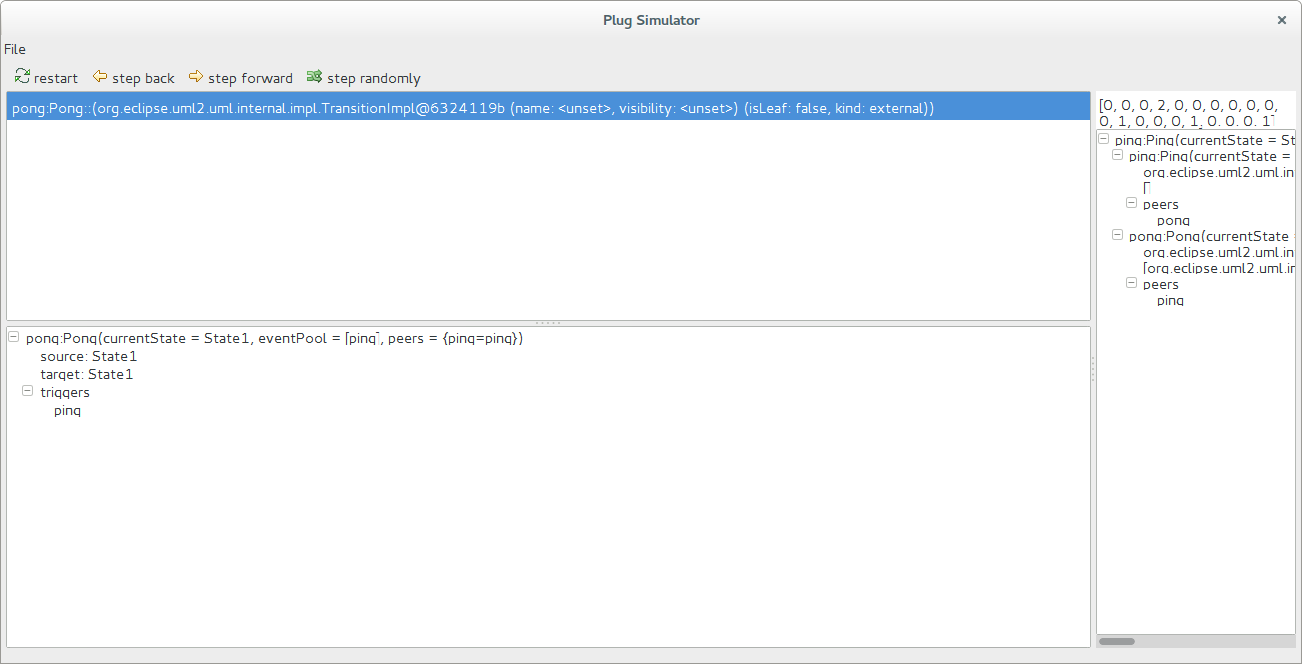
\includegraphics[width=\textwidth]{simulateur}
    \captionof{figure}{Teodorov Simulator Interface}
  \end{minipage}\hfill
  \begin{minipage}{0.45\textwidth}
    The Teodorov simulator is a simulator of uml diagram.

    This simulator needs some object:
    \begin{itemize}
    \item A Class diagram
    \item A State Machine diagram for all class
    \end{itemize}
  \end{minipage}

  \transdissolve[duration=0.1]
\end{frame}

\subsection{Explanation about the simulation}
\begin{frame}
  \frametitle{Explanation about the simulation}
  \begin{figure}[h]
    \centering
    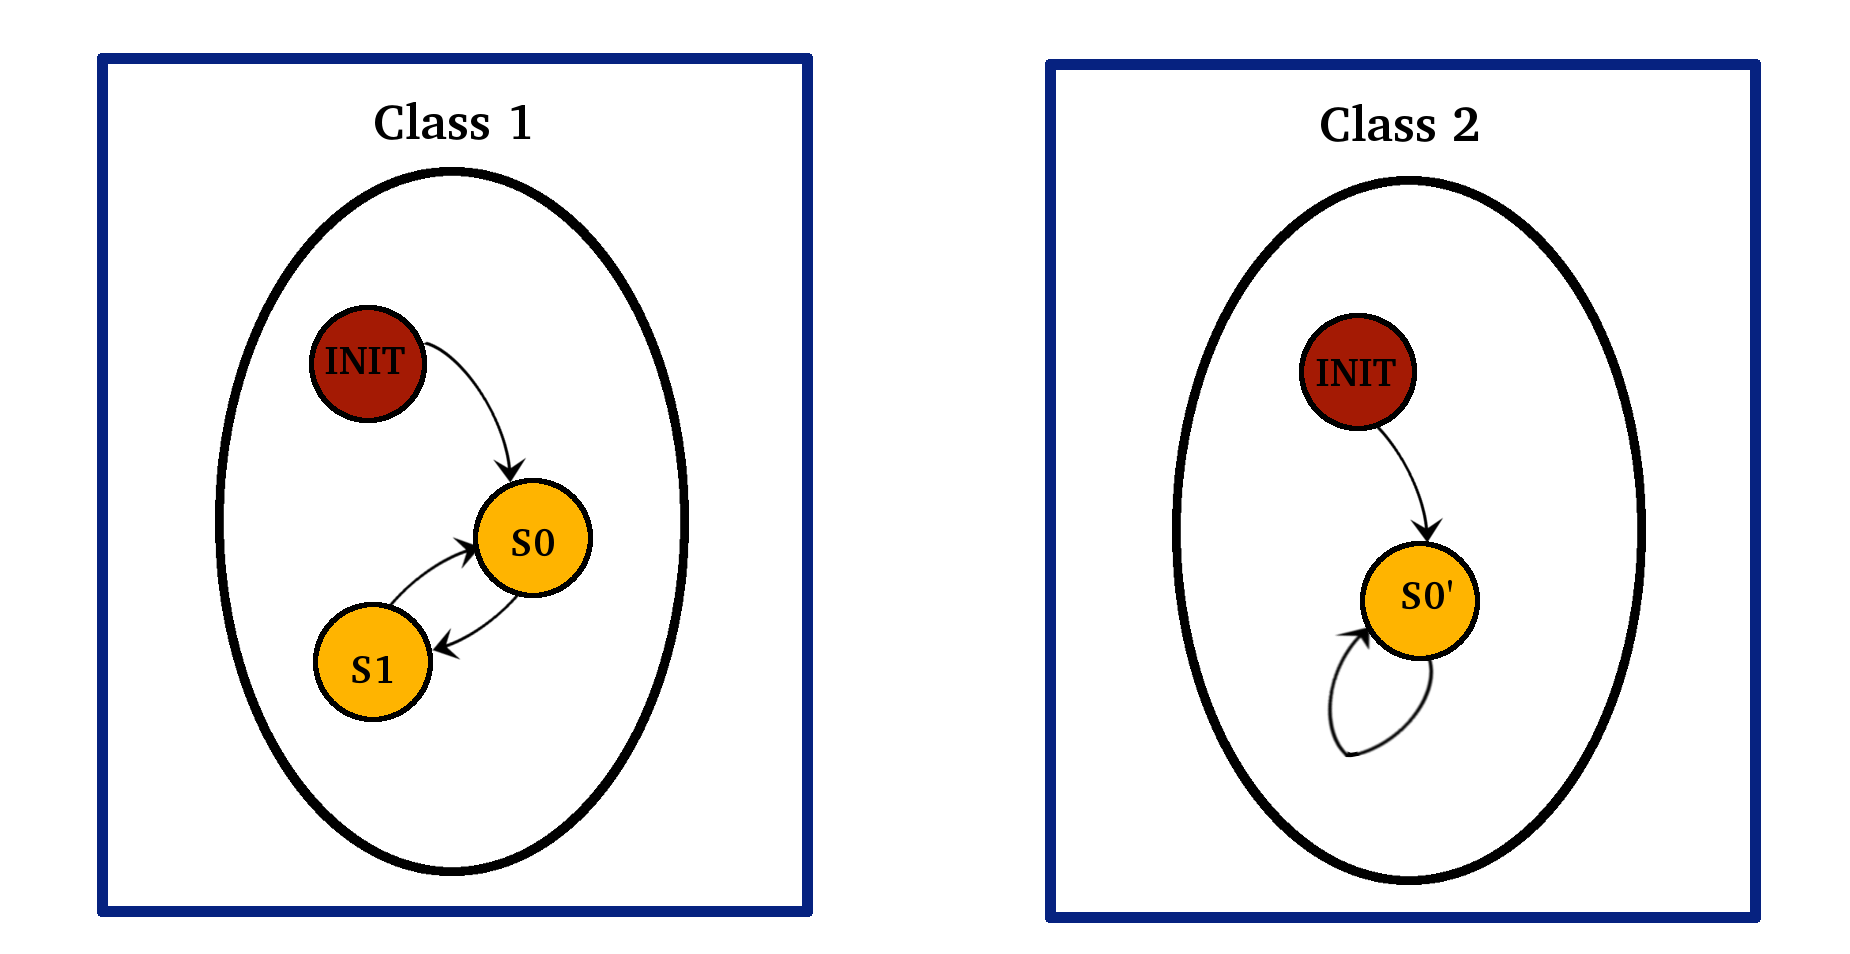
\includegraphics[width=\textwidth]{simulation}
    \caption{Representation of the most important elements of the simulator}
  \end{figure}

  \transdissolve[duration=0.1]
\end{frame}


\subsection{UML Designer}
\begin{frame}
  \frametitle{UML Designer}
  \begin{minipage}{0.45\textwidth}
    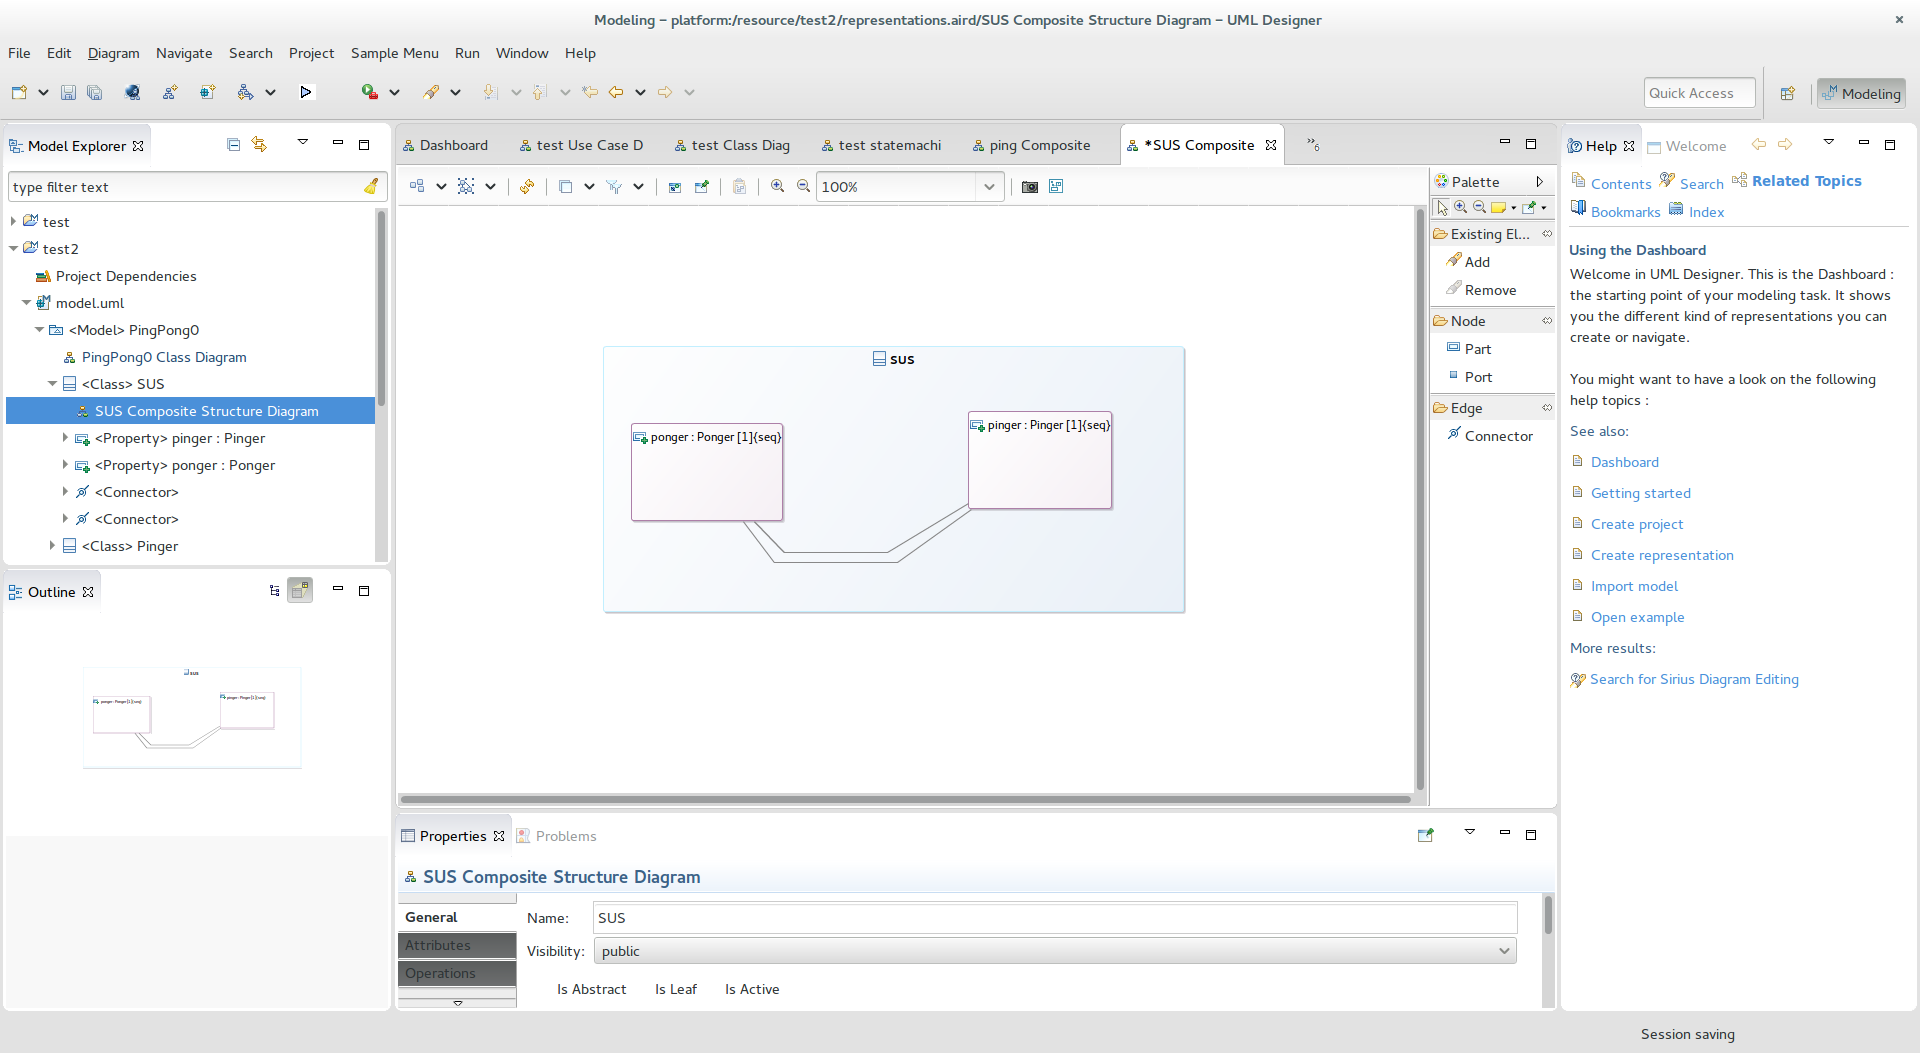
\includegraphics[width=\textwidth]{umldesigner}
    \captionof{figure}{UML Designer Interface}
  \end{minipage}\hfill
  \begin{minipage}{0.45\textwidth}
    UML Designer is an open-source tool to edit and visualize UML2 models created by the French company: \textit{Obeo}. The project is licensed under the EPL%\footnote{Eclipse public license}
  \end{minipage}
  \transdissolve[duration=0.1]
\end{frame}

\subsection{UML Designer kernel}
\begin{frame}
  \frametitle{UML Designer kernel}
  \begin{minipage}{0.45\textwidth}
    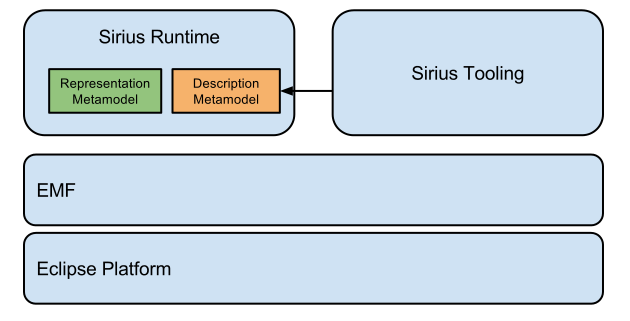
\includegraphics[width=\textwidth]{sirius_archi}
    \captionof{figure}{Sirius kernel \cite{sirius}}
  \end{minipage} \hfill
  \begin{minipage}{0.45\textwidth}
    UML Designer is based on:
    \begin{itemize}
    \item UML Designer plugin
    \item Sirius
    \item EMF
    \item Eclipse kernel
    \end{itemize}
  \end{minipage}

  \transdissolve[duration=0.1]
\end{frame}



%%%%%%%%%%%%%%%%%%%%%%%%%%%%

\section{Presentation of the project}

\subsection{Goals}
\begin{frame}
  \frametitle{Goals}
  \begin{figure}[h]
    \centering
    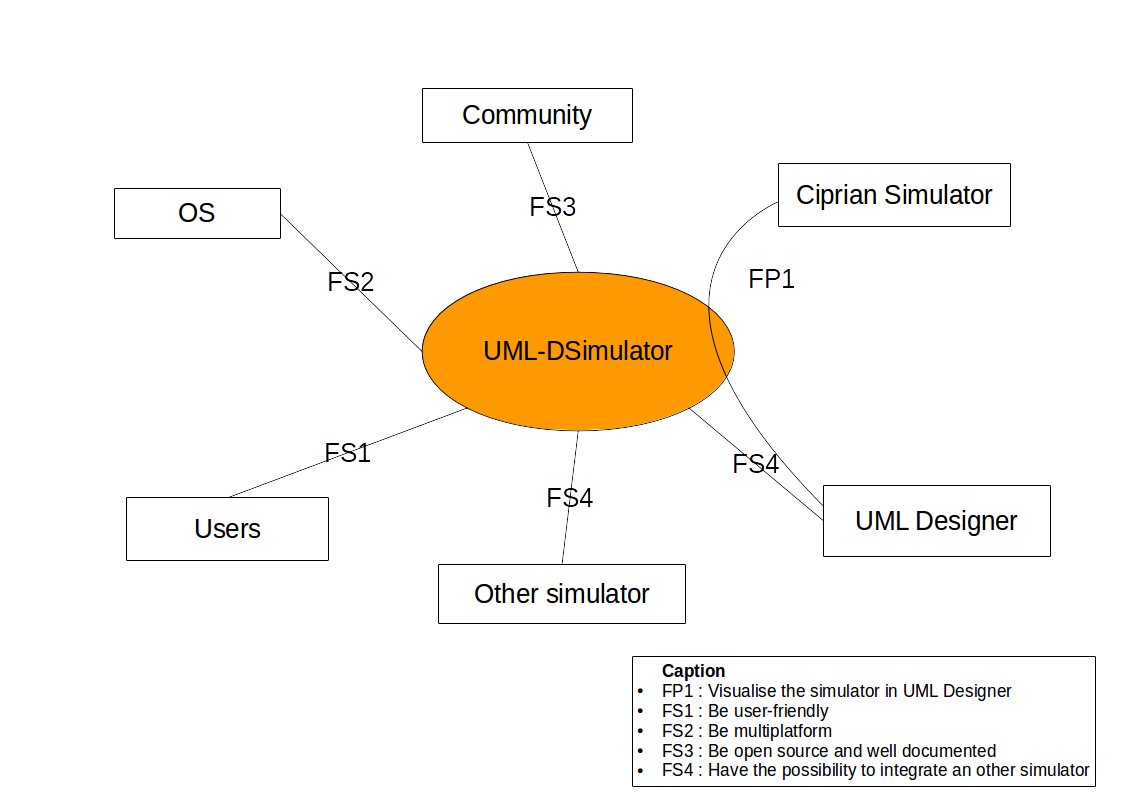
\includegraphics[width=0.9\linewidth]{pieuvre}
    \caption{Octopus Diagram}
  \end{figure}
  \transdissolve[duration=0.1]
\end{frame}

\subsection{Organization}
\begin{frame}
  \frametitle{Organization}
  \begin{figure}
    \begin{minipage}[h]{0.45\linewidth}
      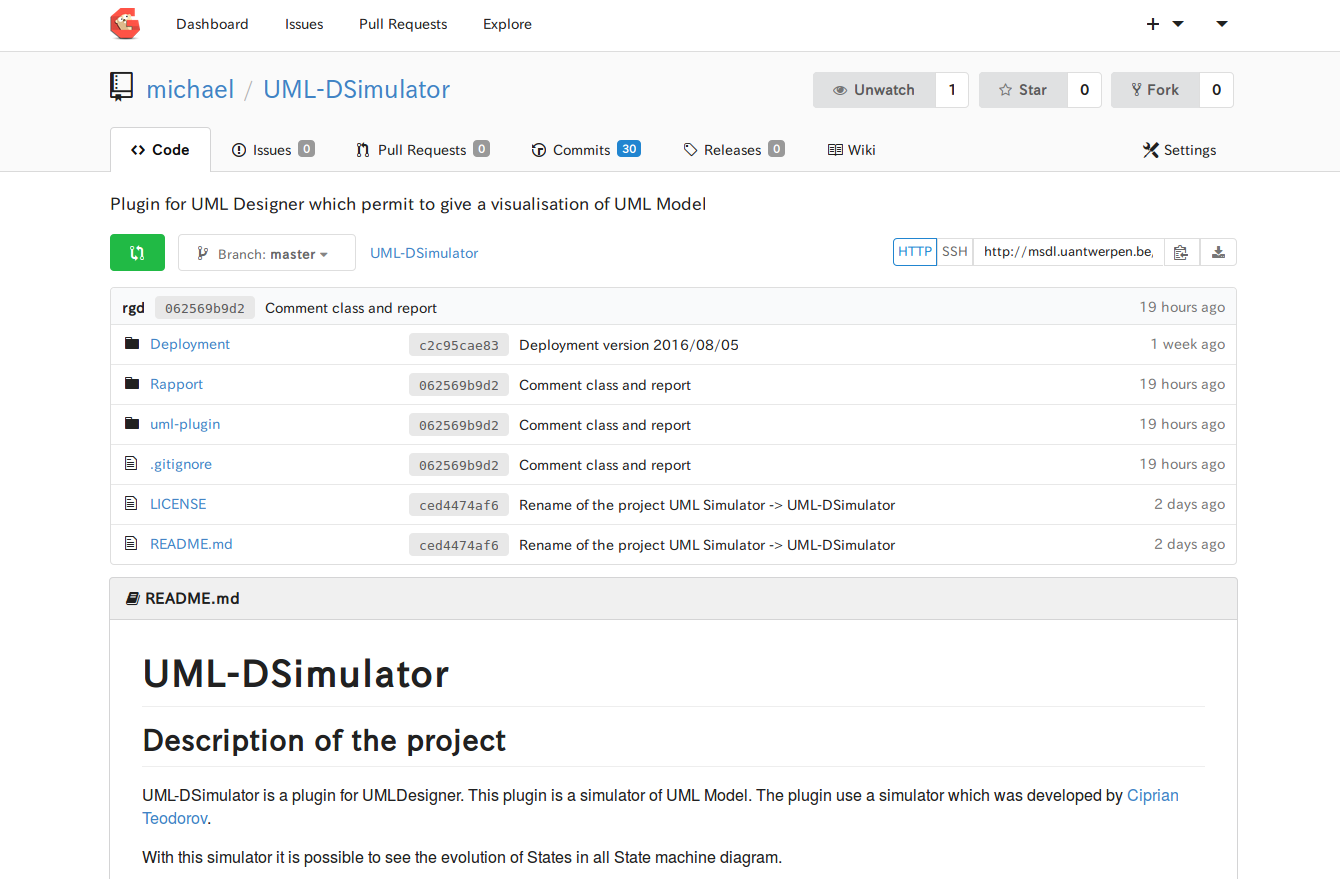
\includegraphics[width=\linewidth]{git}
      \caption{Git repository}
    \end{minipage}
    \hfill
    \begin{minipage}[h]{0.45\linewidth}
      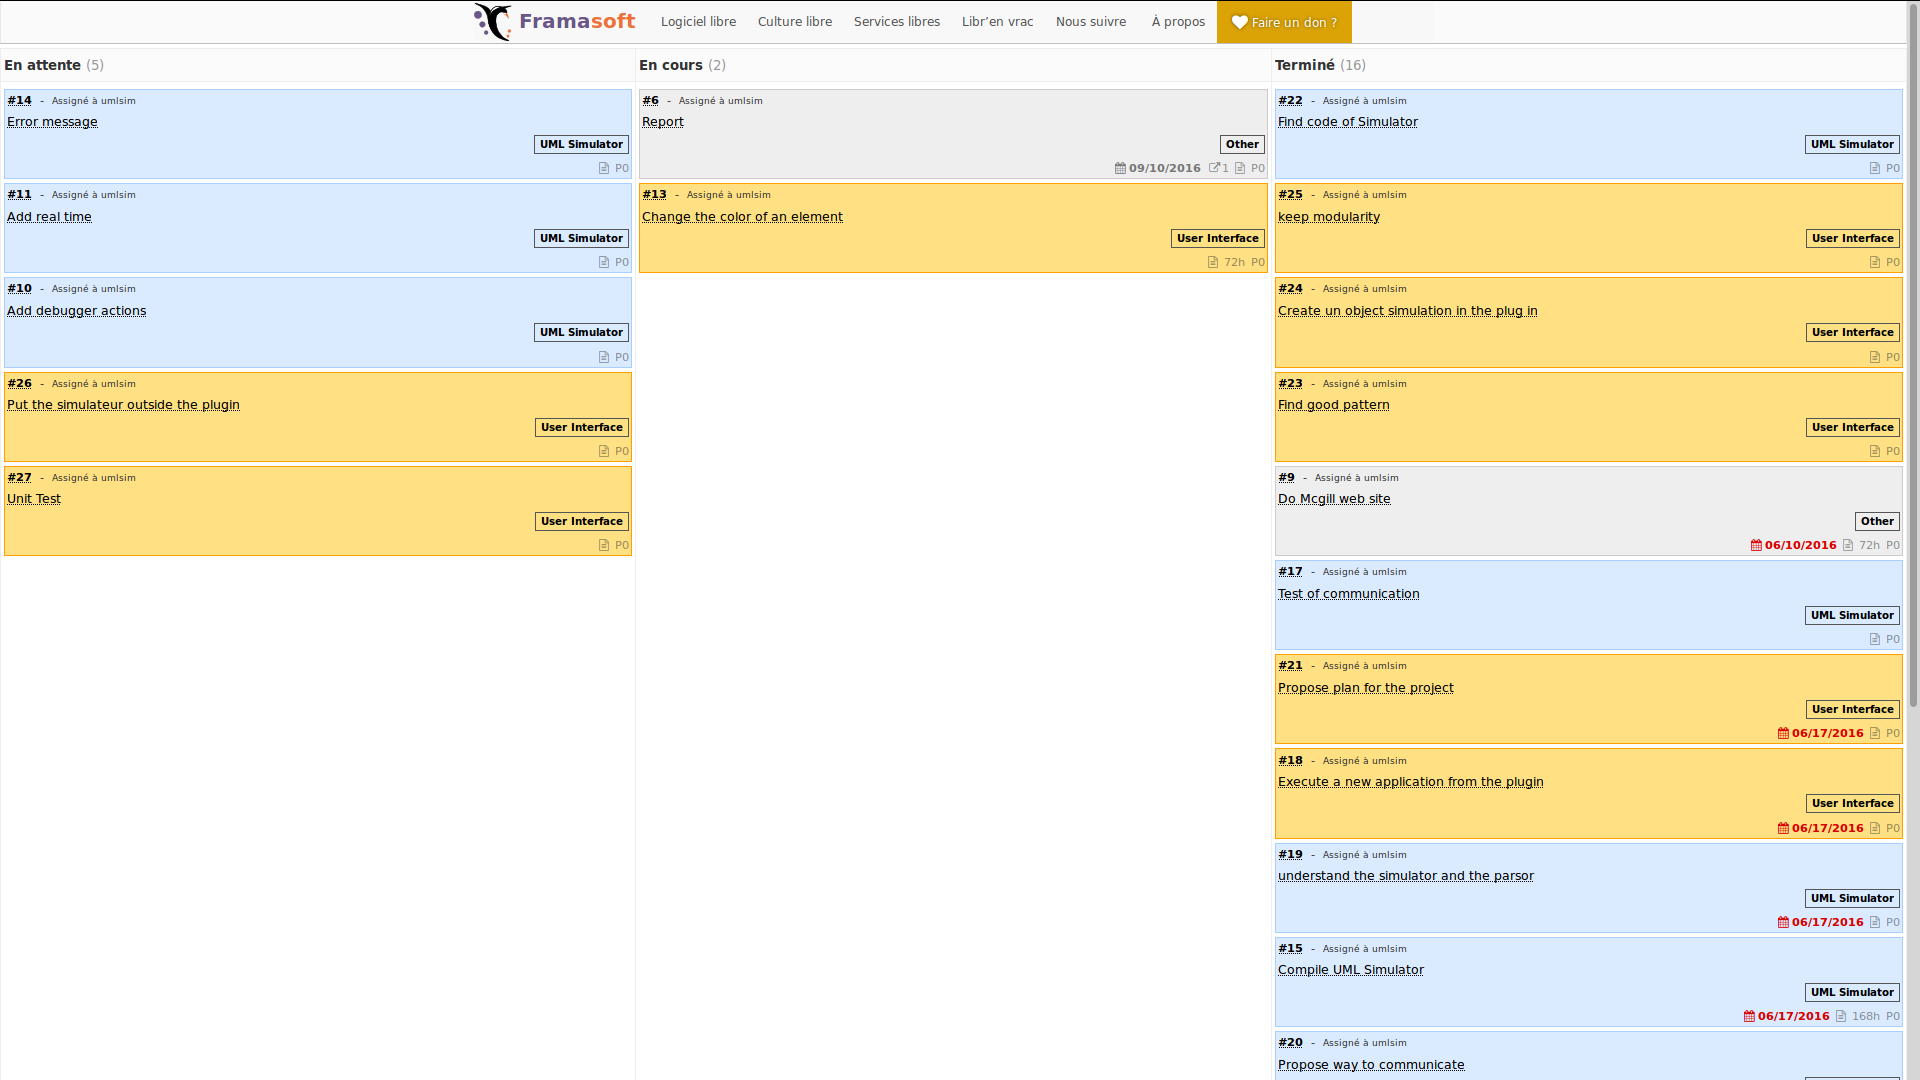
\includegraphics[width=1.1\linewidth]{framaboard}
      \caption{Kanban diagram}
    \end{minipage}
  \end{figure}
  \transdissolve[duration=0.1]
\end{frame}

\subsection{Planning}
\begin{frame}
  \frametitle{Planning}
  \begin{figure}[h]
    \centering
    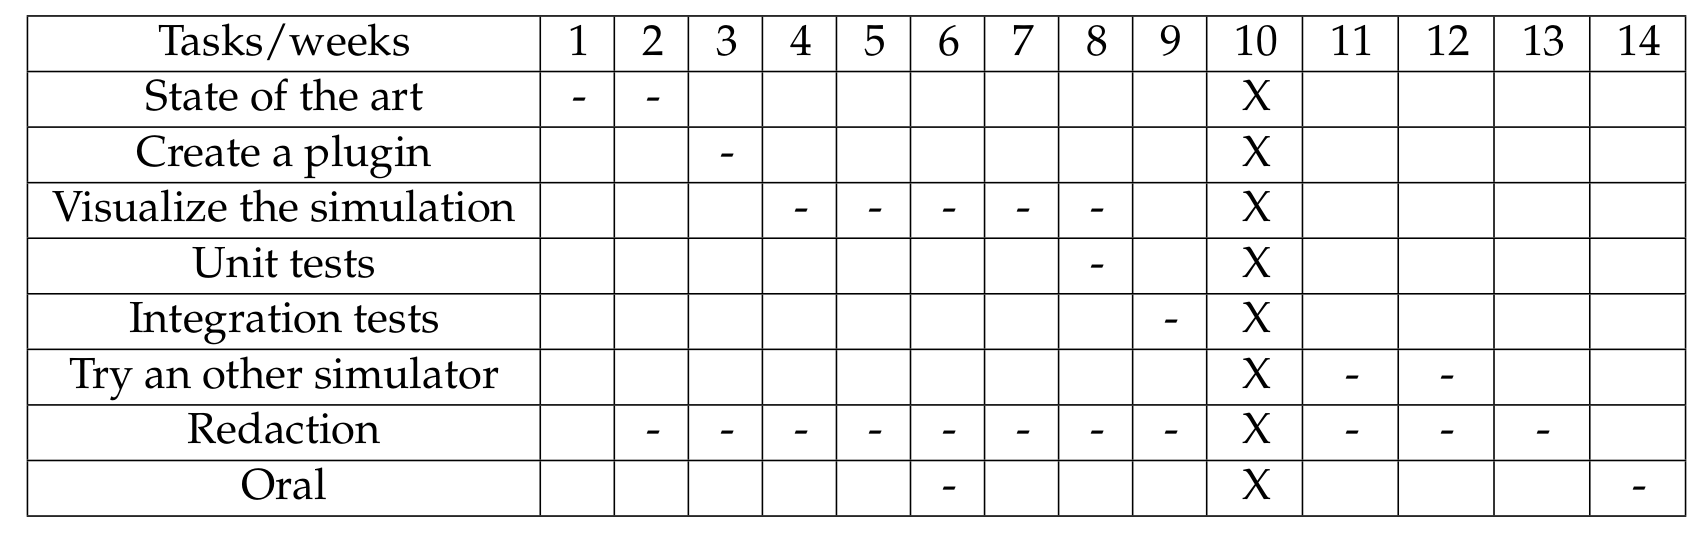
\includegraphics[width=\linewidth]{calendar}
    \caption{Planning}
  \end{figure}

  \transdissolve[duration=0.1]
\end{frame}


%%%%%%%%%%%%%%%%%%%%%%%%%%%%%
\section{Results of the internship}

\subsection{Technical choice}
\begin{frame}
  \frametitle{Technical choice}
  \begin{figure}[h]
    \centering
    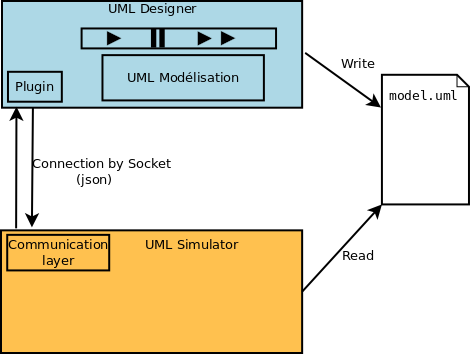
\includegraphics[width=0.8\textwidth]{project}
    \caption{Overview of the project}
  \end{figure}

  \transdissolve[duration=0.1]
\end{frame}

\subsection{Plugin}
\begin{frame}
  \frametitle{Plugin}
  \begin{figure}[h]
    \centering
    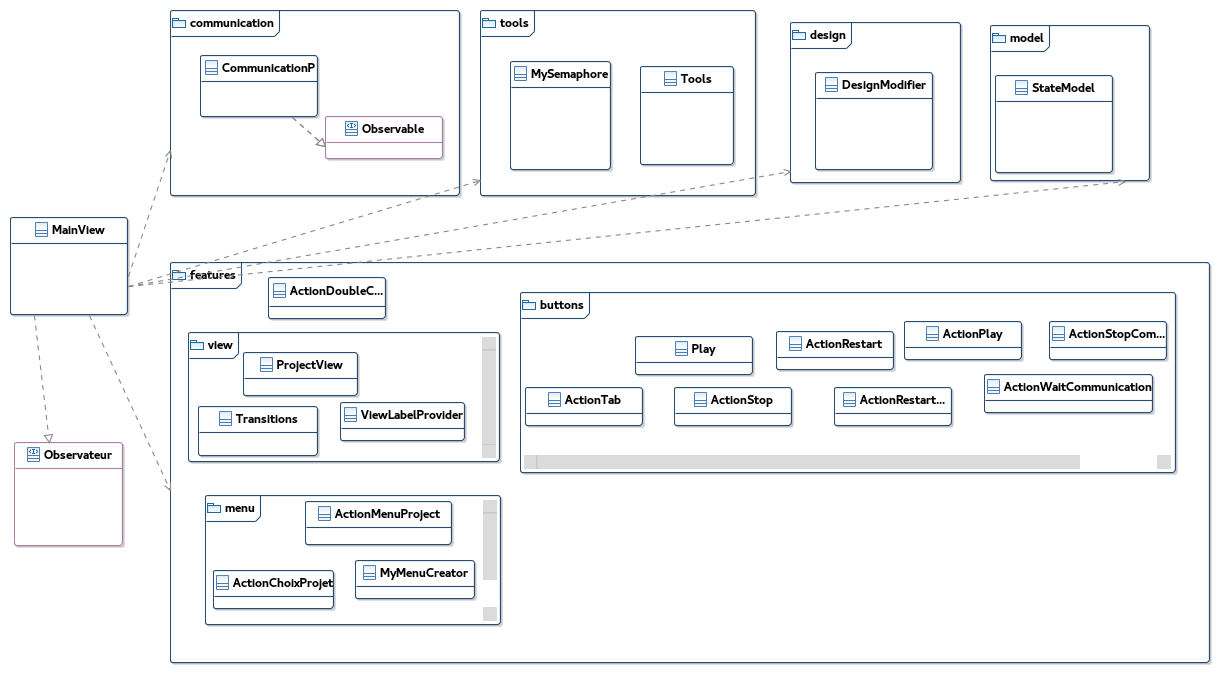
\includegraphics[width=\linewidth]{umlClassDiagram}
    \caption{UML class diagram}
  \end{figure}

  \transdissolve[duration=0.1]
\end{frame}

\subsection{Functionality implemented}
\begin{frame}[label=done]
  \frametitle{Functionality implemented}
  \begin{alertblock}{Work done}
    \begin{itemize}
    \item Integration of the Ciprian simulator in UML Designer
    \item Visualization of the simulation on State Machine Diagram and Class Diagrams
    \item Possibility to choose the next step
    \item Possibility to change the simulator
    \item A play mode
    \item Take care about instances creation
    \item Possibility to chose the instance visible
    \end{itemize}
  \end{alertblock}
  \hyperlink{todo}{\beamerbutton{13/07/2016}}
  \transdissolve[duration=0.1]
\end{frame}


\subsection{SCCD}
\begin{frame}
  \frametitle{SCCD}
  \begin{figure}[h]
    \centering
    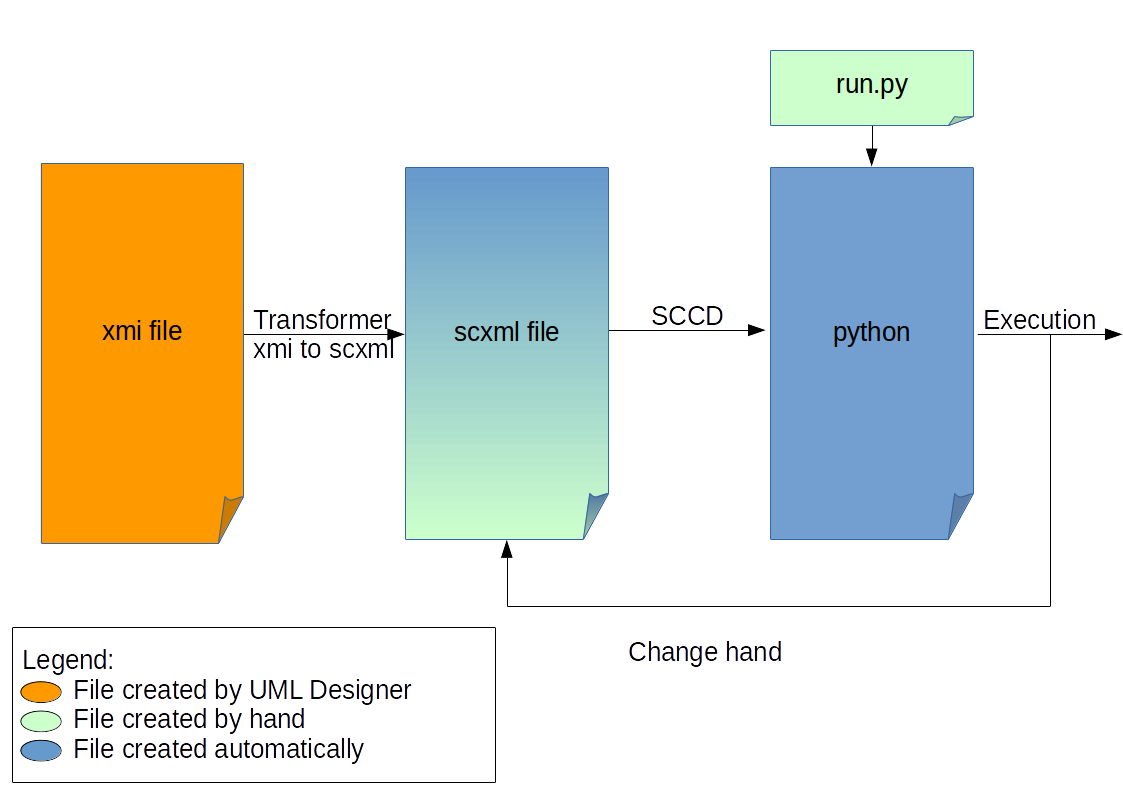
\includegraphics[width=\linewidth]{scxml}
    \caption{scxml creation}
  \end{figure}
  \transdissolve[duration=0.1]
\end{frame}

\subsection{Tests}
\begin{frame}
  \frametitle{Tests}
  \begin{figure}[h]
    \begin{minipage}[h]{0.45\linewidth}
      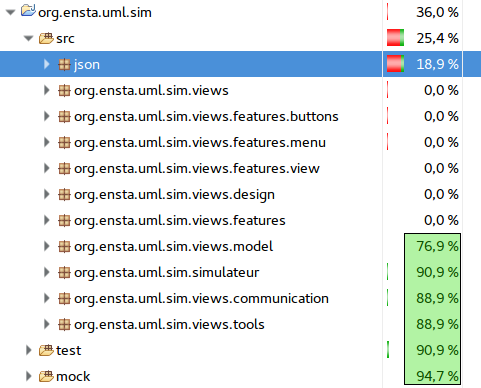
\includegraphics[width=\linewidth]{coverage_zoom}
      \caption{Coverage of my Unit Tests}
    \end{minipage}
    \hfill
    \begin{minipage}[h]{0.45\linewidth}
      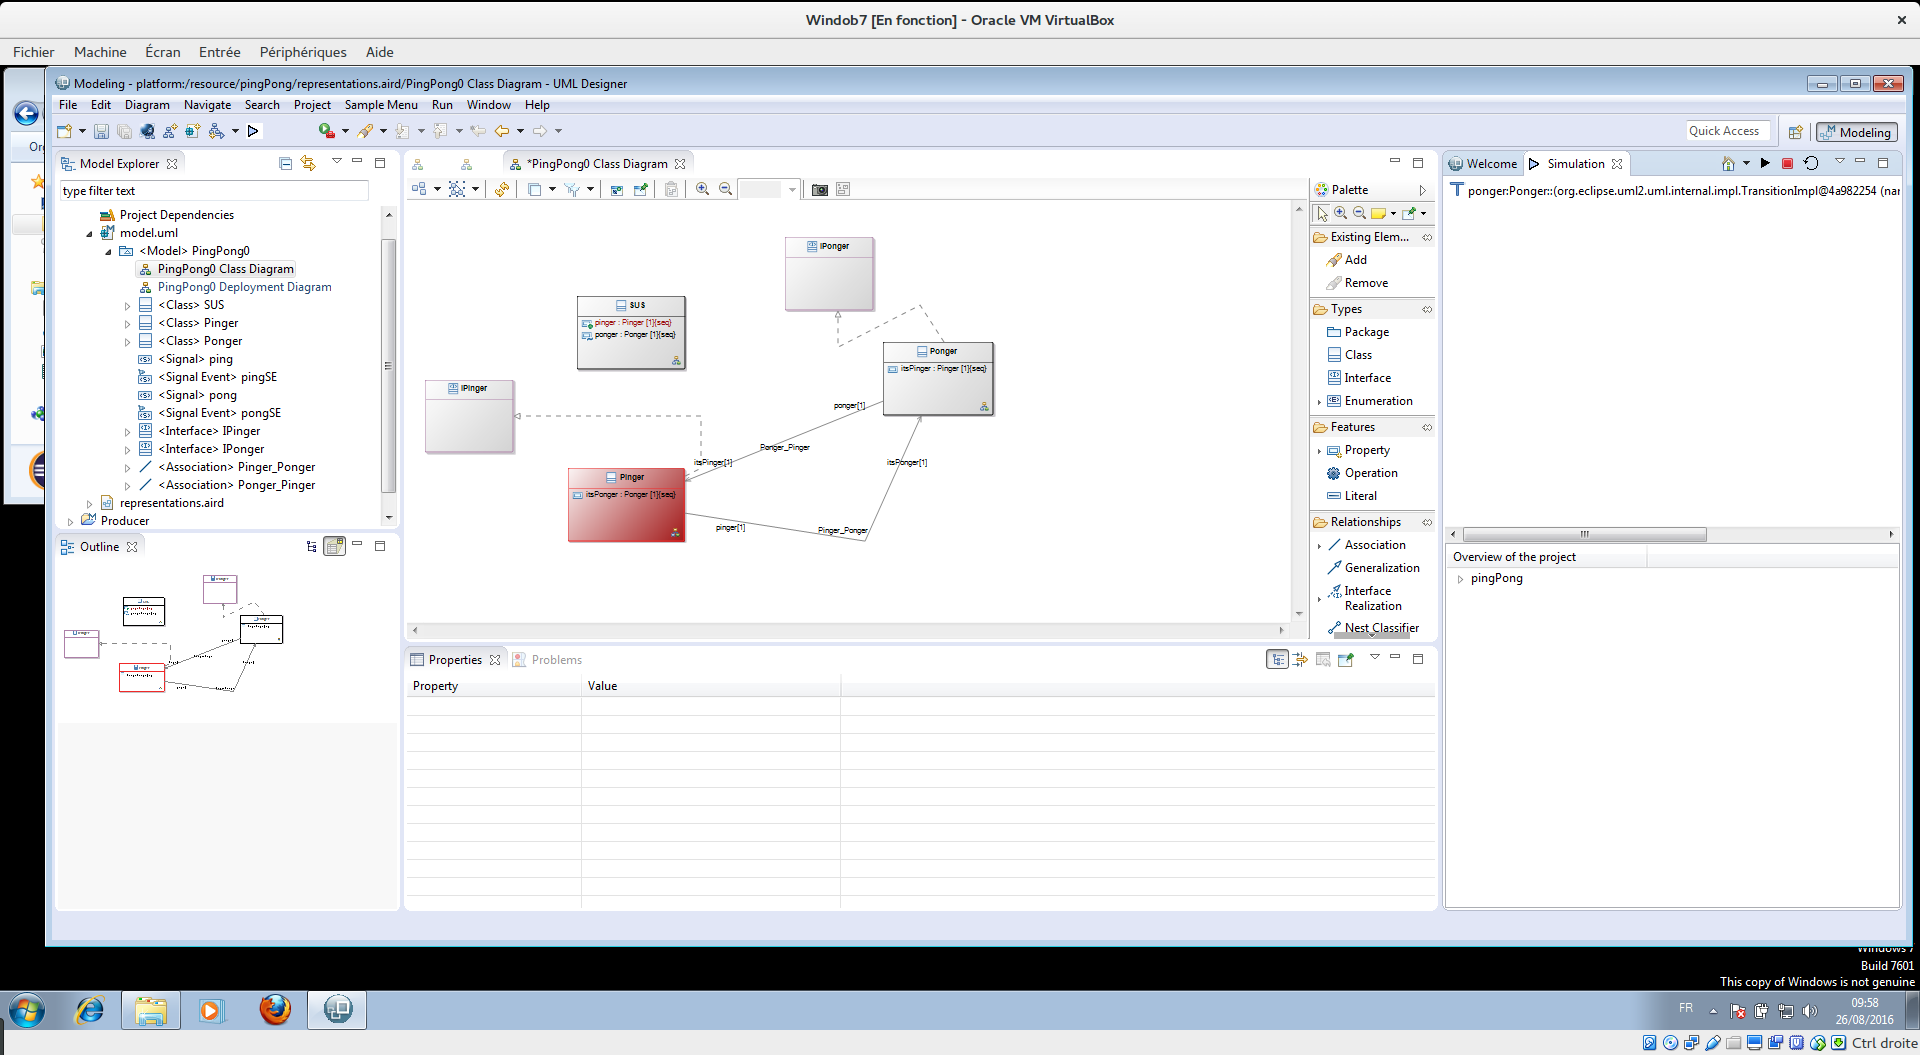
\includegraphics[width=\linewidth]{windows}
      \caption{Screen-shot of the Windows virtual machine}
    \end{minipage}
  \end{figure}

  \transdissolve[duration=0.1]
\end{frame}
%%%%%%%%%%%%%%%%%%%%%%%%%%%%%%%%

\section[Contribution]{Contribution of this internship for my professional project}

\subsection{Contribution of this internship}
\begin{frame}
  \frametitle{Contribution of this internship}
  \begin{alertblock}{Acquisition}
    \begin{itemize}
    \item Discover how work a research laboratory
    \item Learn lot of things about SCCD and Statechart
    \item Improve my scholarship abilities
    \end{itemize}
  \end{alertblock}
  \begin{alertblock}{Encountered difficulties}
    \begin{itemize}
    \item Understand how works UML Designer and the Ciprian Simulator
    \item Find the good API
    \item Block by the Simulator
    \end{itemize}
  \end{alertblock}
  \transdissolve[duration=0.1]
\end{frame}




%%%%%%%%%%%%%%%%%%%%%%%%%%%%%
\section{Conclusion}
\begin{frame}
  \frametitle{Conclusion}
  \begin{alertblock}{To conclude}
    \begin{itemize}
    \item The project has some trouble due to the simulator
    \item Need some improvement in Debugging fields
    \item It can't be use by everybody
    \end{itemize}
  \end{alertblock}
  \begin{alertblock}{But, I am happy because...}
    \begin{itemize}
    \item The plugin is stable, modular and documented
    \item I learn a lot of things, and I overwhelm myself
    \item Mr Champeau is satisfied of my works
    \end{itemize}
  \end{alertblock}
  \transdissolve[duration=0.1]
\end{frame}



\begin{frame}[allowframebreaks]
  \frametitle{Demonstration}
  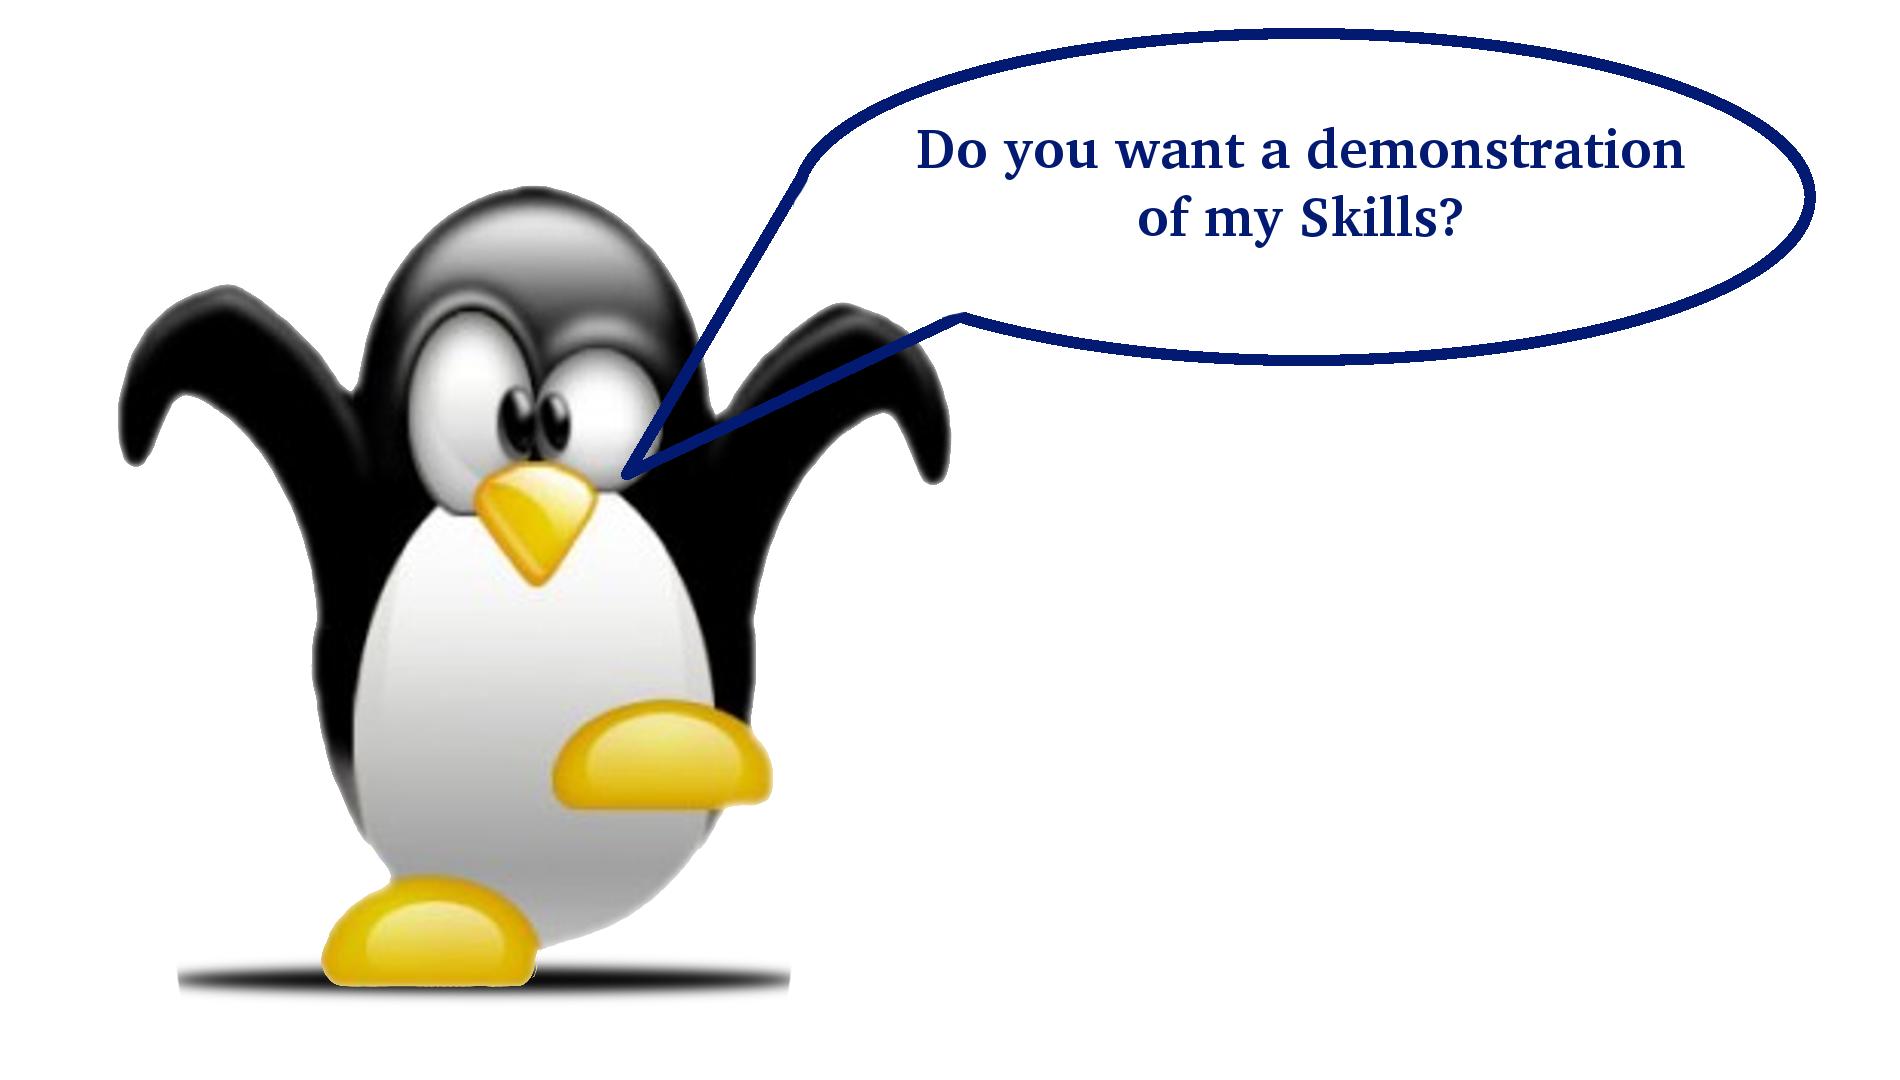
\includegraphics[width=\textwidth]{tux_demo_en}
  \transdissolve[duration=0.1]
\end{frame}


\begin{frame}[allowframebreaks]
  \frametitle{Bibliography}
  \nocite{*}
  \bibliography{biblio}
  \transdissolve[duration=0.1]
\end{frame}


\begin{frame}
  \frametitle{Questions?}

  \begin{center}
    
\includegraphics[width=0.7\textwidth]{tux_ask}
  \end{center}
  \transdissolve[duration=0.1]
\end{frame}

\appendix
\subsection{MSDL organization}
\begin{frame}
  \frametitle{MSDL organization}
  \begin{figure}[h]
    \centering
    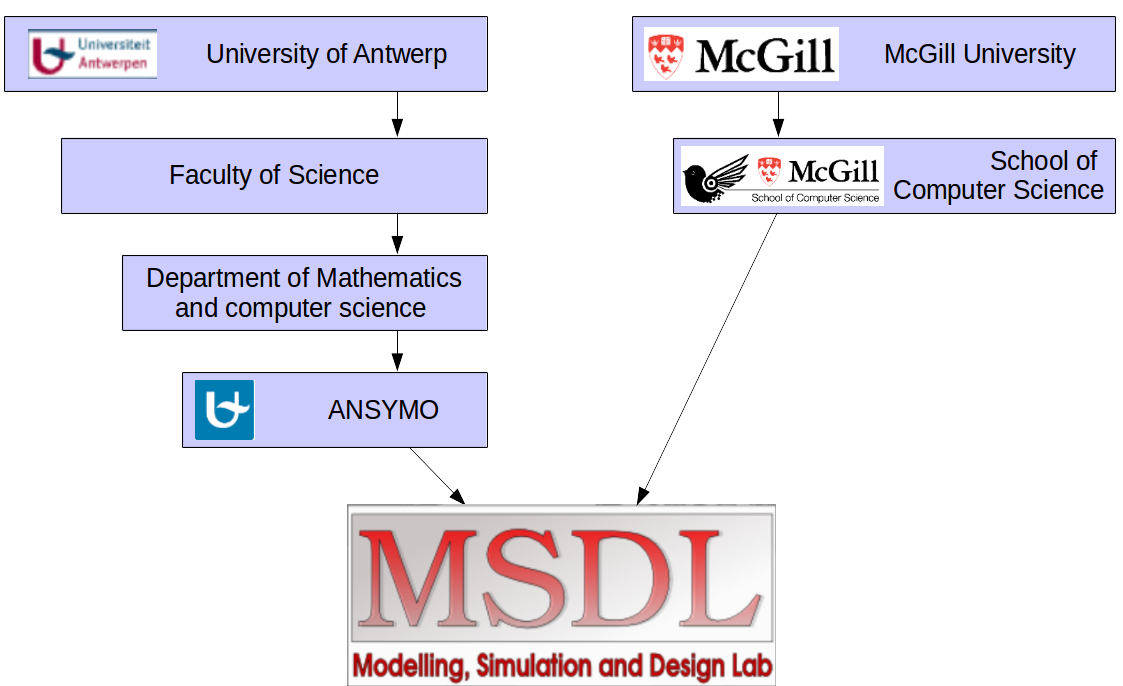
\includegraphics[width=\linewidth]{msdl_organisation}
    \caption{Position of MSDL}
  \end{figure}
  \transdissolve[duration=0.1]
\end{frame}

\subsection{How to write plugin}
\begin{frame}
  \frametitle{How to write plugin}
  \begin{figure}[h]
    \begin{minipage}[h]{0.45\linewidth}
      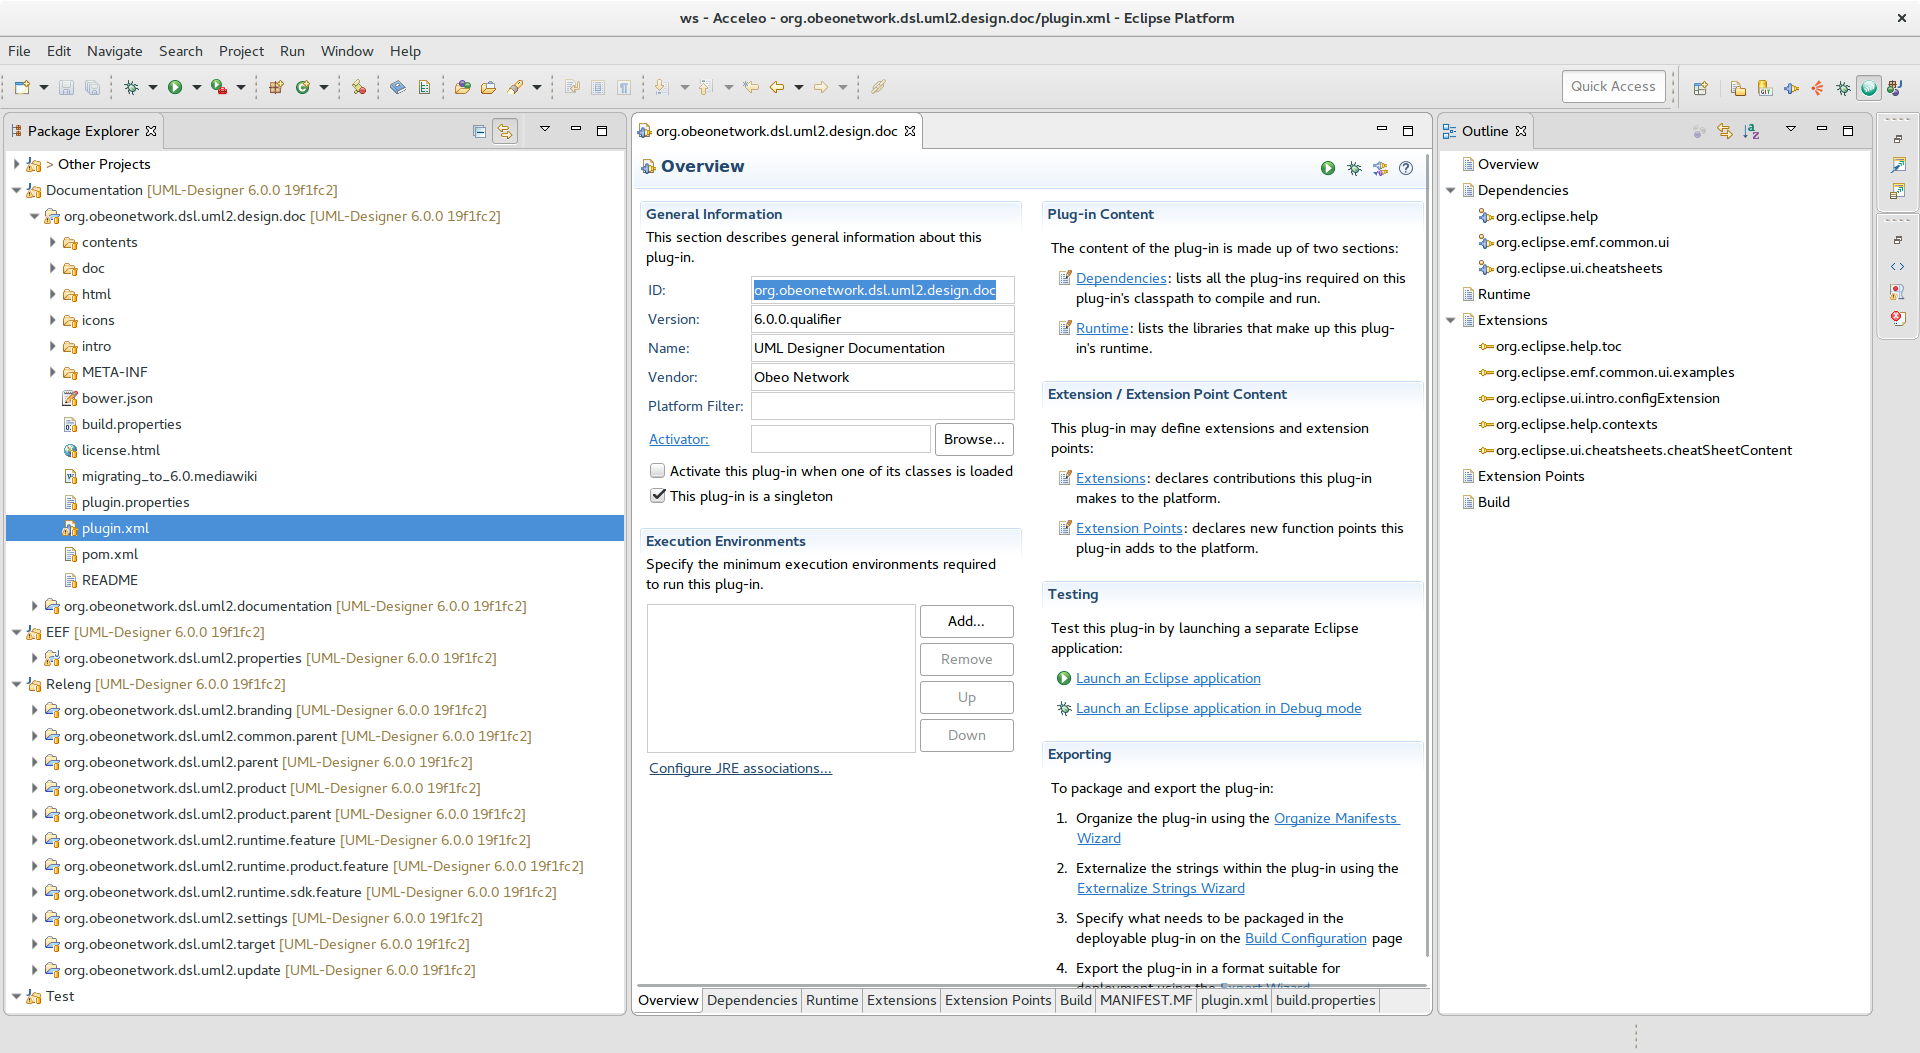
\includegraphics[width=\linewidth]{eclipse}
      \caption{Eclipse environment}
    \end{minipage}\hfill
    \begin{minipage}[h]{0.45\linewidth}
      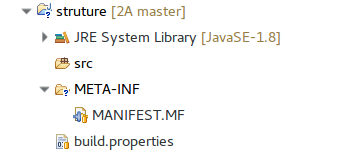
\includegraphics[width=\linewidth]{structure_plugin}
      \caption{Structure of an eclipse plugin}
    \end{minipage}
  \end{figure}
  \transdissolve[duration=0.1]
\end{frame}

\subsection{Why Socket}
\begin{frame}
  \frametitle{Why Socket}
  \begin{tabular}{|p{0.45\textwidth}||p{0.45\textwidth}|}
    \hline
    \textbf{Advantages}&\textbf{Drawback}\\
    \hline
    Work with every language (python, java, ...) & Message need to be formatted\\
    \hline
    Allow communications enter process which don't use the same language& Not very fast\\
    \hline
    Work on all platform (Windows, Linux, OSX)&\\
    \hline
  \end{tabular}

  \transdissolve[duration=0.1]
\end{frame}


\subsection{TODO (13/07/2016)}
\begin{frame}[label=todo]
  \frametitle{TODO (13/07/2016)}
  \begin{alertblock}{Planned}
    \begin{itemize}
    \item Give the choice of the simulator
    \item Show states in the State Machine diagrams
    \item Improve the User experience
    \end{itemize}
  \end{alertblock}
  \begin{alertblock}{If I have time...}
    \begin{itemize}
    \item Create a Sequence Diagram automatically
    \item Create a Debug view
    \item Show real time
    \end{itemize}
  \end{alertblock}
  \hyperlink{done}{\beamerbutton{Functionality implemented}}
  \transdissolve[duration=0.1]
\end{frame}

\end{document}

%%% Local Variables:
%%% mode: latex
%%% TeX-master: t
%%% End:
